% This must be in the first 5 lines to tell arXiv to use pdfLaTeX, which is strongly recommended.
\pdfoutput=1
% In particular, the hyperref package requires pdfLaTeX in order to break URLs across lines.

\documentclass[11pt]{article}

\usepackage[a4paper, total={6in, 8in}]{geometry}
\usepackage{lineno}
\linenumbers

\usepackage{caption,subcaption}

\usepackage{mystyle}

\usetikzlibrary{calc,patterns,angles,quotes}    
\usetikzlibrary{decorations.pathmorphing}
\tikzset{snake it/.style={decorate, decoration=snake}}

\usepackage{natbib}
\bibliographystyle{abbrvnat}
\usepackage{hyperref}

% Standard package includes
\usepackage{times}
\usepackage{latexsym}

% For proper rendering and hyphenation of words containing Latin characters (including in bib files)
\usepackage[T1]{fontenc}
% For Vietnamese characters
% \usepackage[T5]{fontenc}
% See https://www.latex-project.org/help/documentation/encguide.pdf for other character sets

% This assumes your files are encoded as UTF8
\usepackage[utf8]{inputenc}


\title{An Introduction to an Application of the Implicit Function Theorem}

\author{Justin Chiu \\
  Cornell Tech \\
  \texttt{jtc257@cornell.edu}}

\begin{document}
\maketitle
\begin{abstract}
Gradient-based learning forms the foundation of modern machine learning,
and automatic differentiation allows ML practitioners to easily compute gradients.
While automatic differentiation only costs a constant multiple of the time and space
required to evaluate a function, it has its limitations.
In particular, when evaluating a function itself is expensive,
the direct application of automatic differentiation is infeasible.
In this report, we review the implicit function theorem (IFT)
and its use in reducing the cost of computing gradients in scenarios where
function evaluation is expensive,
focusing on the application of implicit differentiation to variational inference.
\end{abstract}

\section{Introduction}
\label{sec:intro}
Gradient-based learning underpins many of the recent successes in machine learning,
particularly advances involving neural networks.
The key to the success of gradient-based methods is automatic differentiation (AD),
which greatly increases the development speed of machine learning research by
allowing practitioners to circumvent the error-prone and time-consuming process
of computing gradients manually.
AD operates by reducing functions into compositions of atomic operations,
for which we have a library of derivatives for,
and composing those derivatives via the chain rule.
The underlying concept behind AD is that a program's execution trace is a valid
and powerful representation of a function \citep{griewank2008autodiff}.

Storing the execution trace of a program allows AD systems to easily compute derivatives.
However, longer execution traces can quickly consume a large amount of memory.
Consider an iterative method, such as gradient descent,
whose execution trace takes the form of an unrolled loop:
Given an initial point $\theta = x_0$,
iterates $x_1, x_2, ..., x_{K}$ are produced by running the gradient descent
update for $K$ iterations.
In order to compute $\frac{dx_K}{d\theta}$ using AD,
we have to store all the $x_k$ iterates
as well the computation used to produce them.
Thus, the memory complexity of storing this execution trace scales linearly in the
number of iterations $K$ as well as the dimensionality of the iterates $x_k$.
For large $K$, this can be infeasible.
One method for overcoming the space complexity's dependence on the number of iterations $K$ in
the above example is to use the implicit function theorem (IFT),
letting you throw away $x_1$ through $x_{K-1}$
while still being able to compute the derivative $\frac{dx_{K}}{dx_0}$.

In this report, we will cover the use of the IFT
as a method for dealing with the space complexity of AD in certain cases.
We will focus on applying the IFT to differentiating the solutions to optimization problems
\citep{optnet,agrawal2019diffcvx}.

\section{Related Work}
There are a variety of methods for overcoming the space limitations of AD,
of which we only mention three: checkpointing, reversible computation, and implicit differentiation.
The first method, checkpointing, improves space complexity at the cost of time \citep{griewank2008autodiff}.
Rather than storing all intermediate computation,
checkpointing instead recomputes values when needed.
This can result in a large slowdown,
and also requires careful choosing of which computationals subgraphs to checkpoint.
A second method is an improvement upon checkpointing, called reversible computation \citep{maclaurin2015reversible,gomez2017reversible},
which improves space complexity at the cost of expressivity, but not speed.
Reversible computation ensures that the gradient with respect to (wrt) the
input depends only on the output,
allowing the input to be discarded during function evaluation.
This is typically accomplished by ensuring that the input is easily reconstructed from the output,
restricting the expressivity of layers.
A third method is implicit differentiation,
which potentially improves space complexity at the cost of stronger assumptions.
Implicit differentiation relies on the implicit function theorem (IFT),
which gives conditions under which derivatives can be computed independent of
intermediate computation.
The primary condition is the characterization of the output as the solution
to a system of equations.

One application of implicit differentiation is bilevel optimization.
Bilevel optimization problems are, as implied by the name,
optimization problems with another nested inner optimization problem embedded within.
Methods for solving bilevel optimization typically proceed iteratively.
For every iteration when solving the outer optimization problem,
we must additionally solve an inner optimization problem.

The application we focus on in this report is expressing individual layers of a neural network declaratively
as the solution of an optimization problem \citep{optnet,agrawal2019diffcvx,gould2019declarative}.
This allows models to learn, without heavy manual specification, the constraints of the problem
in addition to the parameters of the objective.
An example of this is learning to play Sudoku from only input-output pairs.
While the unstructured models struggle to satisfy the hard constraints of Sudoku,
OptNet is able to succeed to a reasonable degree \citep{optnet}.

Other applications that can be formulated as bilevel optimization problems are
hyperparameter optimization, metalearning, and variational inference.
Hyperparameter optimization formulates hyperparameter tuning as a bilevel optimization problem,
as for each hyperparameter configuration a new model must be trained as the inner loop
\citep{maclaurin2015reversible,lorraine2019implasso,lorraine2019hoift,bertrand2020implicit}.
Gradients must then be propagated through the inner training loop to the outer hyperparameter
loop.
Similarly, metalearning learns the parameters of a model such that the model is able to quickly
be adapted to a new task via gradient descent \citep{finn2017maml,rajeswaran2019imaml}.
This is accomplished by differentiating through the learning procedure of each new task.
Finally, a variant of variational inference follows a very similar format:
semi-amortized variational inference (SAVI) aims to learn a model that is able to provide
a good initialization for variational parameters that are subsequently updated iteratively
to maximize a lower bound objective \citep{kim2018savi}.
This is also accomplished by differentiating through the iterative optimization procedure
applied to the variational parameters during inference.

In all the above applications, the inner-loop optimization problem is solved
with an iterative method, except in rare, simple cases.
The IFT reduces the memory footprint of automatic differentiation,
which would otherwise be difficult to scale.

\section{The Implicit Function Theorem}
The implicit function theorem (IFT) has a long history, as well as many applications
in a wide variety of fields such as economics and differential geometry.
For an overview of the history of the IFT and some of its classical applications
in mathematics and economics,
see the book by \citet{iftbook}.

\begin{figure}
%\begin{minipage}{0.48\textwidth}
\centering
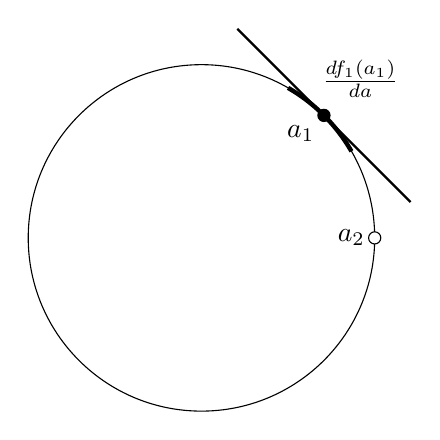
\begin{tikzpicture}[scale=1.1]
\draw (0,0) circle (2);

\node at ($2*({sqrt(2) / 2}, {sqrt(2) / 2})$) (x)[below left] {$a_1$};
\draw[fill=black] ($2*({sqrt(2) / 2}, {sqrt(2) / 2})$) circle (2pt);

% neighbourhood 
\draw[ultra thick] ($2*({sqrt(2) / 2}, {sqrt(2) / 2})$) arc(45:60:2);
\draw[ultra thick] ($2*({sqrt(2) / 2}, {sqrt(2) / 2})$) arc(45:30:2);


% tangent
%\path (2,1) node[point,label={180:P}] {P} at +(120:2){};
\node at ($2*({sqrt(2) / 2 + .21}, {sqrt(2) / 2 + .21})$) {$\frac{df_1(a_1)}{da}$};
\draw[thick] ($2*({sqrt(2) / 2 + -.5}, {sqrt(2) / 2 + .5})$) --
    ($2*({sqrt(2) / 2 + .5}, {sqrt(2) / 2 -.5})$);

% singular point
\node at (2,0) (x2)[left] {$a_2$};
\draw[fill=white] (2,0) circle (2pt);
\end{tikzpicture}
\caption{
\label{fig:circle}
A circle, defined by the relation $a^2 + b^2 - 1 = 0$.
While we cannot differentiate the relation directly,
we can compute derivatives at the point $a_1$ using the local parameterization $f_1(a)=\sqrt{1-b^2}$ that holds
in a neighbourhood around $a_1$, visualized as an arc.
We cannot use the same parameterization at $a_2$ as the derivative is undefined.
In general, the IFT is most useful in cases more complicated than the unit circle,
where local parameterizations are too complex to write down.
}
\end{figure}


\subsection{What is the IFT?}
Consider the unit circle,
governed by the relation $F(a,b) = a^2 + b^2 - 1 = 0$,
which can be interpreted as a system of equations.
As $F$ fails the vertical line test, we cannot write $b$ as a function of $a$ globally.
This prevents us from taking derivatives, for example $\frac{db}{da}$.
However, we can use local parameterizations: $f_1(a) = \sqrt{1-b^2}$ if $b > 0$
or $f_2(a) = -\sqrt{1-b^2}$ if $b<0$.
Note that the local parameterizations hold only within a neighbourhood of a particular
solution $(a,b)$.
These local parameterizations then allow us to take derivatives $\frac{db}{da}$
at particular points $(a,b)$ using the corresponding parameterization.
See Fig.~\ref{fig:circle} for an illustration.
The IFT generalizes this example, and formalizes the conditions under which there exist
continuous local parameterizations for a given relation or system of equations.

While the unit circle in this example has very simple local parameterizations,
in general local parameterizations can be more complicated: For example,
a series of iterative updates is a local parameterization.
Additionally, the IFT does not give the form of the local parameterizations;
it only guarantees the existence of one around a point and a way to compute its derivative.
The local parameterization is left implicit, hence the `implicit' in IFT.

Formally, given a system of equations $F(\theta, x) = \mathbf{0}_m$,\footnote{
We denote vectors and matrices of all 1s and 0s by $\mathbf{1}_S$
and $\mathbf{0}_S$, where $S$ denotes the shape, i.e. $\mathbf{0}_m\in\R^m$.
}
and a solution point $(\theta,x) \in \R^n\times\R^m$,
the IFT gives sufficient conditions under which $x$ can locally be written as a function
of just the parameters $\theta$ within a neighbourhood of the solution point $(\theta,x)$.\footnote{
Going back to the unit circle example, the local parameterizations were only valid around
a particular $(a,b)$ point.
In that example, $a$ was the parameter and $b$ the solution.
}
We refer to this function $x^*(\theta) = x$ as a solution mapping,
and informally refer to $x$ as a solution, as $\theta$ are parameters.
These conditions are as follows:
\begin{enumerate}
\item We have a solution point $(\theta, x)$ that satisfies the system of equations
    $F(\theta, x) = 0$.
\item $F$ has at least continuous first derivatives: $F \in \mcC^1$.
\item The Jacobian matrix of $F$ wrt $x$ evaluated at the solution point $(\theta,x)$ is nonsingular:
    $\det \frac{d F(\theta,x)}{d x} \neq 0$.
\end{enumerate}
Given these conditions hold for $F,\theta,$ and $x$, the IFT
asserts the existence of the implicit solution mapping $x^*(\theta):\R^n\to\R^m$,
and that the derivative of the solution mapping is given by
$\frac{d x^*(\theta)}{d\theta} = -[\frac{dF(\theta,x)}{dx}]^{-1}
    \frac{d F(\theta,x)}{d\theta}$.

{\color{red} still searching for a good intuitive explanation.}

\subsection{How is the IFT useful?}
As mentioned in Sec.~\ref{sec:intro}, the IFT is useful for saving memory when performing
automatic differentiation.
The main benefit of the IFT is that once we have a solution to a system of equations,
we can forget about how we obtained that solution but still compute derivatives.

\begin{figure}
\centering
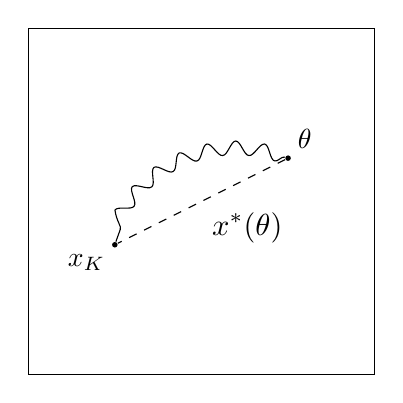
\begin{tikzpicture}[scale=1.1]
%\draw (0,0) circle (2);
\draw (-2,-2) rectangle (2,2);

\node[circle,fill=black, minimum size=2pt, inner sep=0] (x) at (1,.5) {};
\node at (x)[above right] {$\theta$};
\node[circle,fill=black, minimum size=2pt, inner sep=0] (y) at (-1,-.5) {};
\node at (y)[below left] {$x_{K}$};

\draw[snake it] (x)      to [bend right = 45] (y);
\path[dashed] (x) edge (y) node[midway,below right]{$x^*(\theta)$};

\end{tikzpicture}
\caption{
\label{fig:optift}
An example relationship between the parameters $\theta$,
solution $x_{K}$ after $K$ iterations of an iterative method,
and implicit function $x^*(\theta)$ of the IFT.
The rectangle depicts a space which, in this example,
contains both $\theta$ and $x_K$.
This is not necessary for the IFT, but simplifies illustration.
The parameters $\theta$ provide an initial point, which is then iteratively refined
into solution $x_{K}$, shown by the squiggly line.
If $x_{K}$ satisfies the conditions of the IFT, then the IFT both
guarantees the existence of the implicit solution mapping $x_K = x^*(\theta)$
(dashed line)
and tells us how to compute $\frac{dx^*(\theta)}{d\theta}$.
This is useful if the iterative procedure (squiggly line), is too expensive
to store in memory for use in automatic differentiation.
}
%\end{minipage}
\end{figure}

In particular, we will show how to compute derivatives of the solution of an optimization problem
wrt parameters of the problem without storing intermediate computations,
as illustrated in Fig.~\ref{fig:optift}.
We will use the optimality criteria of the optimization problem to define a system of equations,
then apply the IFT to compute the Jacobian of the solution wrt the parameters.
This methodology allows us to use the solution to an optimization problem
as the output of a layer within a neural network,
as done in OptNet \citep{optnet}.
%We will then discuss the problem addressed by this method in OptNet.

Afterwards, we will cover an application of the IFT to speeding up variational inference.

\section{Embedding Optimization inside a Neural Network}
As an introductory example,
we will replace the softmax layer of a neural network with an equivalent function
defined as the output of an optimization problem, then derive derivatives using the IFT.
We will start by reviewing softmax and its expression as an optimization problem.
After checking the conditions of the IFT hold, we can then compute derivatives.
Since the Jacobian of softmax is known, we can directly verify that the IFT gives
the correct answer.

\subsection{Learning via the chain rule}
Before we get into the details of softmax, we first motivate the learning problem.
Neural networks consist of stacks of layers,
all of which take the output of the previous layer as input.
In order to train neural networks we rely on reverse mode AD, or backpropagation.
Reverse mode AD propagates error information backward through the network via the chain rule.
Key to this process is the Jacobian matrix of each layer, the matrix of partial derivatives
of the layer's outputs wrt its inputs.

Given a function $F:\R^n\times\R^m\to\R^m$, we denote the Jacobian evaluated at
the point $(\theta,x)\in\R^n\times\R^m$ as
\begin{equation*}
\frac{dF(\theta,x)}{d(\theta,x)} = \begin{bmatrix}
    \frac{dF(\theta,x)}{d\theta} &\frac{dF(\theta,x)}{dx} 
\end{bmatrix},
\end{equation*}
where we have the matrix of partial derivatives
\begin{equation*}
\frac{dF(\theta,x)}{d\theta} = \begin{bmatrix}
    \frac{dF_1(\theta,x)}{d\theta_1} & \cdots & \frac{dF_1(\theta,x)}{d\theta_n} \\
    \vdots & \ddots & \vdots \\
    \frac{dF_m(\theta,x)}{d\theta_1} & \cdots & \frac{dF_m(\theta,x)}{d\theta_n} \\
\end{bmatrix},
\end{equation*}
and similarly for $\frac{dF(\theta,x)}{dx}\in\R^{m\times m}$.

In order to embed an optimization layer inside a neural network,
we must provide the Jacobian of our layer for use in an AD system.\footnote{
This is a slight simplification. We often need to provide
at least the vector-Jacobian product.
}
With this in mind, we proceed to review softmax and its equivalent formulation
as an optimization problem.

\subsection{Softmax}
Softmax is often used to parameterize categorical distributions within neural networks,
such as in attention layers.
It has its origins in statistical mechanics and decision theory, and functions
as a differentiable surrogate for argmax.

Softmax assumes that we have $n$ items with independent utilities, $\theta \in \R^n$,
which indicate preferences.
Softmax then gives the following distribution over items:
$z_i = \frac{\exp(\theta_i)}{\sum_j \exp(\theta_j)}$, with $z\in\R^n$.
While there is a closed-form equation
for both softmax and its Jacobian,
we use it as an introduction to the mechanism
behind OptNet (and other differentiable optimization layers)
\citep{optnet,agrawal2019diffcvx}.

The output of softmax is the solution of the following optimization problem \citep{gao2018properties}:
\begin{equation}
\label{eqn:softmax-opt}
\begin{aligned}
\textrm{maximize } \quad & z^\top\theta + H(z)\\
\textrm{subject to } \quad & z^\top \mathbf{1} = 1\\
& z_i \geq 0, \forall i,
\end{aligned}
\end{equation}
where $H(z) = -\sum_i z_i \log z_i$ is the entropy.\footnote{
We have taken care to use the variable $z$
for the primal variable of the softmax problem, rather than $x$.
This is because, as we will soon see, the solution point of the resulting system
of equations must also include dual variables.
}
We will refer to this as the softmax problem.\footnote{
Removing the entropy regularization term results in an optimization problem
whose solution is argmax: maximize $z^\top\theta$, subject to $z^\top\mathbf{1}_n=1$
and $z \succeq 0$.
}

Our goal is to compute the Jacobian of softmax
$\frac{dz}{d\theta} = \frac{d\softmax(\theta)}{d\theta}$
using the IFT and the optimization problem above, as an exercise.
Applying the IFT to optimization problems consists of four steps:
\begin{enumerate}
\item Find a solution to the optimization problem.
\item Write down the system of equations.
\item Check that the conditions of the IFT hold.
\item Compute the derivative of the implicit solution mapping wrt the parameters.
\end{enumerate}

We assume the first step has been done for us,
and we have some solution $z$ to the softmax problem.
We will then use the IFT to compute gradients of $z$ wrt the parameters $\theta$
by following the rest of the steps.

\subsection{The KKT conditions determine $F$}
Given an optimization problem, the Karush-Kuhn-Tucker (KKT) conditions
determine a system of equations that the solution must satisfy,
i.e the optimality criteria \citep{kkt-thesis,kkt}.
They are, roughly, stationarity (the gradient should be 0 at a local optima)
and feasibility (the constraints of the problem should not be violated).
For a thorough introduction to the KKT conditions, see chapter 5 of \citet{bv-cvxbook}
or the \href{https://en.wikipedia.org/wiki/Karush-Kuhn-Tucker\_conditions}{Wikipedia article}.\footnote{
If this is your first time seeing the KKT conditions, please check out
one of the suggested references
and make your way back here to flex your new knowledge.
}

We will use the KKT conditions of the softmax problem in
Eqn.~\ref{eqn:softmax-opt} to determine the function $F$ in the IFT.
First, we introduce dual variables $u\in\R,v\in\R^n$ and write out the Lagrangian:
$$\mcL(\theta, z, u, v) = z^\top\theta + H(z) + u(z^\top \mathbf{1} - 1) + v^\top z.$$
We therefore have the solution point $(\theta,z,u,v)$, with parameters $\theta$
and solution $x=(z,u,v)$.
We then have the following necessary conditions for a solution $(z,u,v)$,
i.e. the KKT conditions:
\begin{equation}
\begin{aligned}
\frac{d}{dx} \mcL(\theta, z,u,v) &= \mathbf{0}_n && \textrm{(stationarity)}\\
u(z^{\top} \mathbf{1} - 1) &= 0 && \textrm{(primal feasibility, equality)}\\
\diag(v)z &= \mathbf{0}_{n} && \textrm{(complementary slackness)}\\
z &\succeq \mathbf{0}_n && \textrm{(primal feasibility, inequality)}\\
v &\succeq \mathbf{0}_n && \textrm{(dual feasibility)}
\end{aligned}
\end{equation}
As we only need a system of equations with $2n+1$ equations to
determine the $2n+1$ solution variables $x=(z,u,v)$,
we use the first three conditions: stationary, primal feasibility (equality),
and complementary slackness.

In full, the system of equations $F(\theta, z,u,v) = 0$ is
\begin{equation}
\label{eqn:system}
\begin{aligned}
\theta + -\log(z) - 1 + u\mathbf{1}_n + v &= \mathbf{0}_n\\
u(z^{\top} \mathbf{1}_n - 1) &= 0\\
\diag(v)z &= \mathbf{0}_n.
\end{aligned}
\end{equation}
Note that the first and third equations are vector-valued.

Now we can check the conditions of the IFT.
We assumed we were given an optimal and therefore feasible solution $x=(z,u,v)$
which must satisfy $F(\theta, z,u,v) = 0$,\footnote{
Recall that softmax also has a closed form expression.}
and $F$ has continuous first derivatives, i.e. $F \in \mcC^1$.
All that remains is to check that the Jacobian matrix $\frac{dF(\theta,z,u,v)}{d(z,u,v)}$
(evaluated at the solution point) is non-singular.

The Jacobian $\frac{dF(\theta,z,u,v)}{d(z,u,v)}\in\R^{2n+1\times 2n+1}$ is given by
\begin{equation}
\label{eqn:f-jac}
\frac{dF}{d(z,u,v)}=
\begin{bmatrix}
\diag(z)^{-1} & -\mathbf{1}_n & -I_{n\times n} \\
u\mathbf{1}_n^\top & z^\top\mathbf{1}_n - 1 & 0\\
\diag(v) & 0 & \diag(z)
\end{bmatrix}.
\end{equation}
Since a solution must be feasible, we know that $z^\top\mathbf{1}-1=0$ and $u > 0$.
However, the upper left block, $\diag(z)^{-1}$, contains a divide-by-zero term if
any component $z_i = 0$.\footnote{
This term was obtained by differentiating the entropy
term of the Lagrangian, $H(z) = \sum_i z_i\log z_i$.
While we could use the convention $0\log 0 = 0$,
this does not fix the divide-by-zero issue with the second derivative, which we see here.
}
To avoid this, we consider only strictly positive $z \succ 0$ for the IFT.\footnote{
We saw a similar issue in the unit circle example, where the derivative
$\frac{db}{da}$ was undefined when $a=0$ (see Fig.~\ref{fig:circle}).
}
Given the strict positivity of $z$,
we can deduce that the Jacobian of $F$ is full rank and therefore has nonzero determinant.
This shows that the conditions of the IFT hold.

\subsection{The Jacobian of Softmax}
Now that we have shown that the conditions of the IFT hold,
we can proceed to apply the second part of the IFT in order to compute $\frac{dz}{d\theta}$.
Recall that we have the solution $x = (z,u,v)$; we will switch to $x$ for brevity.
The second part of the IFT tells us that we can compute the Jacobian of the
solution mapping $\frac{dx}{d\theta} = \frac{dx^*(\theta)}{d\theta}
= \left[\frac{dF(\theta,x)}{dx}\right]^{-1}\frac{dF(\theta,x)}{d\theta}$,
then pick out the relevant components.

The second term, $\frac{dF(\theta,x)}{d\theta}$, is simple.
Since $\theta$ only appears in the first vector-valued function of $F$
(see Eqn.~\ref{eqn:system}), we have
\begin{equation}
\label{eqn:df-dtheta}
\frac{dF(\theta,x)}{d\theta} = \begin{bmatrix}
    I_{n\times n}\\
    \mathbf{0}_{(n+1)\times (n+1)}
\end{bmatrix}.
\end{equation}
The large amount of sparsity allows us to skip some computation further down.
\footnote{This sparsity is due to the simple constraints in the softmax problem,
which is no longer available in more general optimization problems.}

Next, we have to invert the Jacobian from Eqn.~\ref{eqn:f-jac}:
\begin{equation}
\label{eqn:dsystem-matrix}
\left[\frac{dF(\theta,x)}{dx}\right]^{-1} = \begin{bmatrix}
\diag(z)^{-1} & -\mathbf{1}_n & -I_{n\times n} \\
u\mathbf{1}_n^\top & x^\top\mathbf{1}_n - 1 & 0\\
\diag(v) & 0 & \diag(z)
\end{bmatrix}^{-1}.
\end{equation}
The remainder of this section is compute-intensive;
feel free to skip ahead to Sec.~\ref{sec:limitations} for a discussion
on the limitations of applying the IFT.
We use the block-wise inversion formula
\begin{equation*}
\begin{bmatrix}
A & B\\
C & D
\end{bmatrix}^{-1} = \begin{bmatrix}
    (A - BD^{-1}C)^{-1} & 0\\
    0 & (D - CA^{-1}B)^{-1}
\end{bmatrix}
\begin{bmatrix}
    I & -BD^{-1}\\
    -CA^{-1} & I
\end{bmatrix},
\end{equation*}
where
\begin{align*}
A = \begin{bmatrix} \diag(z)^{-1} & -\mathbf{1}_n \\ u\mathbf{1}_n^\top & 0 \end{bmatrix}&\qquad\qquad
B = \begin{bmatrix}-I_{n\times n} \\ 0\end{bmatrix}\\
C = \begin{bmatrix}\diag(v) & 0\end{bmatrix} &\qquad\qquad
D = \diag(z).
\end{align*}
However, by complementary slackness, we have $v = 0$,\footnote{
We apply the IFT to solutions where $z\succ 0$ due to a divide-by-zero issue
in $\frac{d^2H(z)}{dz_i^2} = \frac{1}{z_i}$.
}
reducing the above to
\begin{equation*}
\begin{bmatrix}
A & B\\
C & D
\end{bmatrix}^{-1} = \begin{bmatrix}
    A^{-1} & 0\\
    0 & D^{-1}
\end{bmatrix}
\begin{bmatrix}
    I_{(n+1)\times (n+1)} & -BD^{-1}\\
    0 & I_{n \times n}
\end{bmatrix}.
\end{equation*}
As we are interested in computing $\frac{dz}{d\theta}$,
rather than the full derivative $\frac{dx}{d\theta}$ (recall $x = (z,u,v)$),
in addition to the sparsity of $\frac{dF}{d\theta}$, 
we only have to solve for the upper-left $n\times n$ block of $A^{-1}\in\R^{n+1\times n+1}$.
To do so, we will repeat the same block-wise inverse computation.
Let us denote
$$A
= \begin{bmatrix} \diag(z)^{-1} & -\mathbf{1}_n \\ u\mathbf{1}_n^\top & 0 \end{bmatrix}
= \begin{bmatrix}E & F \\ G & H\end{bmatrix}.
$$
First, we compute the Schur complement of $A$,
\begin{equation}
A/E = H - GE^{-1}F = 0 + u\mathbf{1}_n^\top\diag(z)\mathbf{1}_n = uz^\top\mathbf{1}_n.
\end{equation}
Since $z$ is feasible, we have $A/E = u$ due to the equality constraints
($z$ must sum to 1 as a probability mass function).
Then, we have
\begin{equation}
A^{-1} = \begin{bmatrix}
\diag(z)^{-1} & -\mathbf{1}_n\\
u\mathbf{1}^\top_n & 0
\end{bmatrix}^{-1}
=\begin{bmatrix}E & F \\ G & H\end{bmatrix}^{-1}
= \begin{bmatrix}
E^{-1} + E^{-1}F(A/E)^{-1}GE^{-1} & -E^{-1}F(A/E)^{-1}\\
-(A/E)^{-1}GE^{-1} & (A/E)^{-1}
\end{bmatrix}.
\end{equation}
Plugging in,
\begin{equation}
\begin{aligned}
A^{-1} 
&= \begin{bmatrix}
\diag(z) - \diag(z)\mathbf{1}_nu^{-1}u\mathbf{1}^\top_n\diag(z)
    & \diag(z)\mathbf{1}_nu^{-1}\\
-u^{-1}u\mathbf{1}^\top_n \diag(z) & u^{-1}
\end{bmatrix}\\
&= \begin{bmatrix}
\diag(z) - zz^\top
    & u^{-1}z\\
    -z^\top & u^{-1}
\end{bmatrix}.
\end{aligned}
\end{equation}
Pulling out the top-left $n\times n$ block yields
the Jacobian $\frac{d z}{d\theta} = \diag(z) - zz^\top$,
which agrees with directly differentiating softmax \citep{sparsemax}.

Given the formulation of softmax as an optimization problem, we have
successfully shown how to differentiate
the output of softmax wrt the parameters in a solver-agnostic manner using the IFT.
This concludes the exercise of using the IFT to differentiate through the
softmax problem.

%(Example showing build-up of memory from reversible SGD vs IFT would be nice here,
%ie code it up and plot memory consumption / speed. maybe not best example though)

\subsection{Limitations}
\label{sec:limitations}
In order to compute the derivative $\frac{dx}{d\theta}$, we had to invert the Jacobian of $F$.
However, The first part of $F$ (recall from Eqn.~\ref{eqn:system}), the stationarity condition
$\frac{d}{dx}\mcL = 0$,
already involved the Jacobian of the Lagrangian $\mcL$.
In general, this means that in order to apply the IFT to solutions of optimization problems,
we must compute the inverse Hessian of the Lagrangian (or at least a Hessian-vector-product).
The Hessian is a matrix of size $O(n^2)$,
and inverting this would take $O(n^3)$ computation.\footnote{
The number of solution variables scales with the number of primal variables,
but also the number of constraints.
This potentially makes applying the IFT to optimization problems with exponentially
many constraints difficult.
}
Thankfully, there are relatively cheap ways of approximating this computation,
such as with approximate (inverse) Hessian-vector-product techniques
\citep{rajeswaran2019imaml,lorraine2019hoift}.

\subsection{Extensions}
The methods we covered can be extended to variations of argmax problems
other than the softmax problem.\footnote{
The argmax problem is given by maximize $z^\top \theta$, subject to $z^\top\mathbf{1}_n=1$
and $z\succeq 0$.
}
The softmax problem altered the argmax problem by introducing entropy regularization.
Rather than regularizing with entropy, one could instead alter the objective to find
the Euclidean projection of the parameters onto the probability simplex,
resulting in SparseMax \citep{sparsemax}.
While the output of softmax variants often have a closed form expression,
the IFT provides another way of deriving their Jacobians
and could potentially pave the way for differentiating through argmax problems
that do not have closed-form expressions.

More generally, the IFT can be applied to cases where, unlike softmax,
we do not have an explicit functional form (i.e., the unit circle),
and outputs are governed only by a system of equations.
This includes more general optimization problems, such as quadratic programs \citep{optnet}
or other convex optimization problems \citep{agrawal2019diffcvx}.
%as well as the solutions of differential equations \citep{neuralode}.

\section{OptNet}
OptNet generalizes the methodology applied above to the softmax problem by
extending the optimization problems considered,
in particular including parameterized constraints.
This allows us to learn not only the objective, but also the constraints.
Explicitly incorporating families of constraints in models
with optimization layers to allows them to perform well
on tasks with rigid constraints, such as learning to play
Sudoku from only inputs and outputs \citep{optnet}.

\subsection{Quadratic Programs}
OptNet applies the IFT to quadratic programs (QPs) in particular.
As the simplest nonlinear optimization problem,
QPs strike a balance between expressivity and computational tractability \citep{simplex}.
The methodology remains the same as the softmax problem:
Given a QP and a solution,
use the KKT conditions to produce a system of equations then apply the IFT
/ implicit differentiation to compute the derivative of the solution wrt the
parameters of the objective and constraints.

Quadratic programs take the following form:
\begin{equation}
\label{eqn:qp}
\begin{aligned}
\textrm{maximize } \quad & \frac12 x^\top Q x + q^\top x\\
\textrm{subject to } \quad & Ax = b\\
& Gx \leq h,
\end{aligned}
\end{equation}
where we optimize over $x$ and the parameters are $\theta = \set{Q, q, A, b, G, h}$.
Compared to the softmax problem in Eqn.~\ref{eqn:softmax-opt},
we see that the main difference is the learnable parameters in the constraints.
As the application of the IFT is almost identical, we will not cover it in detail.

The second contribution of OptNet was the extension of a state-of-the-art interior point
solver \citep{optnet}, and its adaptation to parallel machines (GPUs) and batch processing.
While outside the scope of this report, see the paper by \citet{optnet} for the details.

\section{Semi-Amortized Variational Inference (POSTPONED / dont read)}
We now apply the IFT to variational inference.

Variational inference has found success in recent applications to generative models,
in particular by allowing practitioners to depart from conjugate models
and extend emission models with expressive neural network components.
The main insight that led to this development is that inference can be amortized through
the use of an inference network.
One approach to variational inference, stochastic variational inference (SVI),
introduces local, independent variational parameters for every instance of hidden variable.
While flexible, the storage of all variational parameters is expensive, and the optimization
of each parameter independently slow \citep{}.
Amortized variational inference (AVI) solves that by instead using a hierarchical process.
Variational parameters are produced hierarchically via an inference network,
which in turn generates the local variational parameters \citep{}.
The resulting local parameters may or may not be subsequently optimized.

Failure to further optimize local variational parameters may result in an amortization gap \citep{}.
Prior work has shown that this gap can be ameliorated by performing a few steps of
optimization on the generated local parameters obtained from the inference network,
and even by propagating gradients through the optimization process.
Optimizing through the inner optimization problem results in semi-amortized variational inference
(SAVI) \citep{}.

As our main motivating example, we will examine whether we can apply the IFT to SAVI.
We will start by formalizing the problem of variational inference for a simple model.

We will start with a model defined by the following generative process,
used by \citet{dai2020vae} to analyze posterior collapse:
\begin{enumerate}
\item Choose a latent code from the prior distribution $z \sim p(z) = N(0, I)$.
\item Given the code, choose an observation from the emission distribution
    $x \mid z \sim p_\theta(x \mid z) = N(\mu_x(z, \theta), \gamma I)$,
\end{enumerate}
where $\mu_x(z, \theta) \equiv \MLP(z, \theta)$ and $\gamma > 0$ is a hyperparameter.
This yields the joint distribution $p(x,z) = p(x\mid z)p(z)$.

Since the latent code $z$ is unobserved, training this model would require optimizing the
evidence $p(x) = \int p(x,z)$.
However, due to the MLP parameterized $\mu_x$, the integral is intractable.
Variational inference performs approximate inference by introducing variational distribution
$q_\phi(z \mid x)$ and maximizing the following lower bound on $\log p(x)$:
\begin{equation}
    \log p(x) - \KL{q(z \mid x) || p(z \mid x)}
    = \Es{q_\phi(z \mid x)}{\log \frac{p_\theta(x,z)}{q_\phi(z\mid x)}} = L(\theta, \phi).
\end{equation}

(Write out objective in full.)

While SVI introduces local parameters for each instance of $z$,
and AVI uses a single $q(z \mid x)$ for all instances,
we will follow the approach of SAVI.
We will perform inference as follows:
For each instance $x$, produce local variational parameter
$z^{(0)} = g(x; \phi)$.
Obtain $z^*$ by solving $\mcL(\theta, z^{(0)}) = 2$, with (local) optima $\ell^*$.
Take gradients through the whole procedure,
i.e. compute $\frac{\partial \ell^*}{\partial \phi}
= \frac{\partial\ell^*}{\partial z^*}\frac{\partial z^*}{\partial z^{(0)}}
\frac{\partial z^{(0)}}{\partial \lambda}$.
The main difficuty lies in computing $\frac{\partial z^*}{\partial z^{(0)}}$.
(Highlight challenge)

In order to avoid the memory costs of storing all intermediate computation performed
in a solver, we will instead apply the IFT.
In order to apply the IFT, we must satisfy the three conditions.
First, we must have a solution point to a system of equations, $F(x_0, z_0) = 0$.
In this setting, we will use the KKT conditions of the optimization problem to define $F$.

\section{Limitations}

\bibliography{bib}

\appendix

\section{Example Appendix}
\label{sec:appendix}

Neural ODEs use reversibility.

\end{document}
